\section{Hough Transformation}

\subsection{Main Theory:}

Hough transform is a voting technique that is used to determine the
``most possible'' lines in the image.

Each line in a 2d image can be represented by:

$y=mx+b,$ where (x,y) is a point in the image space.

Each line in image space can also be represented by a point (m,b) in the
Hough space, where:

$b = -mx + Y$

A single point (x,y) in image space maps to all solutions of
$b = -mx + y$ which corresponds to a line in the hough space.

\begin{figure}[htbp]
\centering
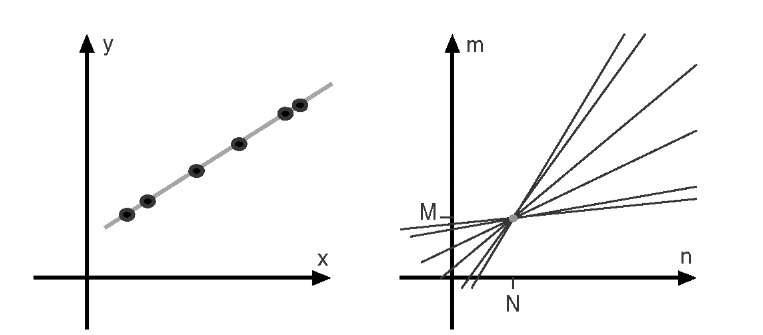
\includegraphics{pics/hough/1.jpg}
\caption{Hough space \label{hough1}}
\end{figure}

If we have two points (x0, y0) and (x1, y1) they'll each correspond to
lines in the hough space. As each point in hough space is a line in the
image space, the point where the lines intersect in hough space, will be
the line in the image space, that contains both points (x0, y0) and (x1,
y1). The solution to:

$b = -mX0 + y0$ and $b = -mx1 + y1$ (intersection between)

\subsubsection{How does it work?}

As input to a Hough algorithm we use a thresholded gradient magnitude
image. (see Fig. \ref{hough3}) This is usually computed by first doing
some soft smoothing, then using a Sobel filter (fig. \ref{hough2}) for
both vertical and horizontal directions.

\begin{figure}[htbp]
\centering
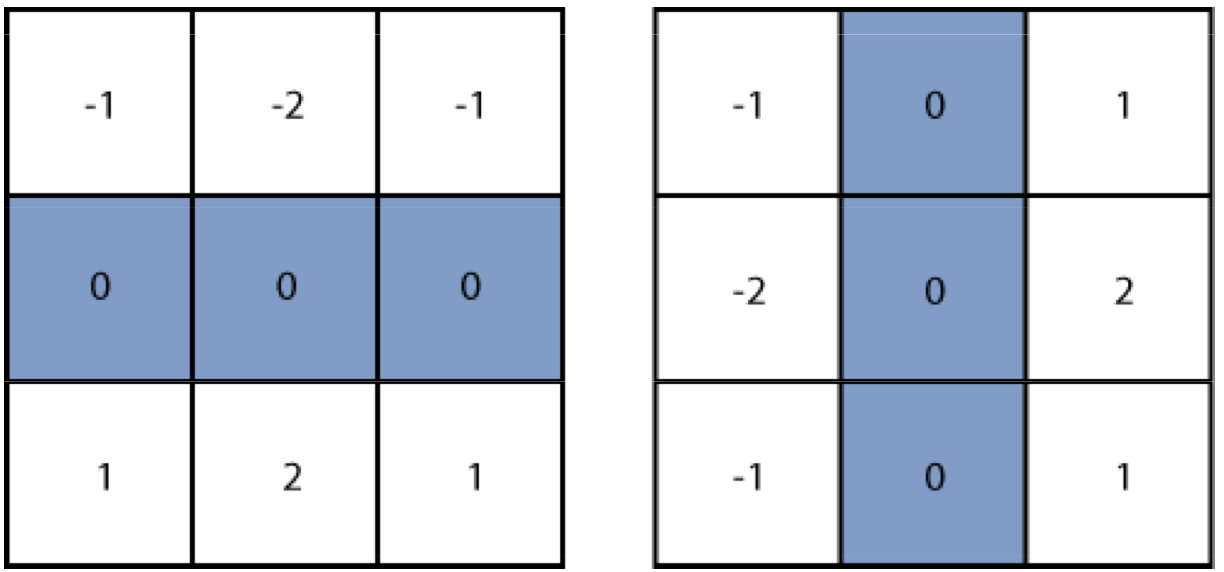
\includegraphics{pics/hough/2.png}
\caption{Sobel kernel \label{hough2}}
\end{figure}

From this image the edge magnitude image is computed, where:

$g(x,y)= sqrt(g2(x,y)+g2(x,y)) is the gradient norm for/in the point (x,y)$

\begin{figure}[htbp]
\centering
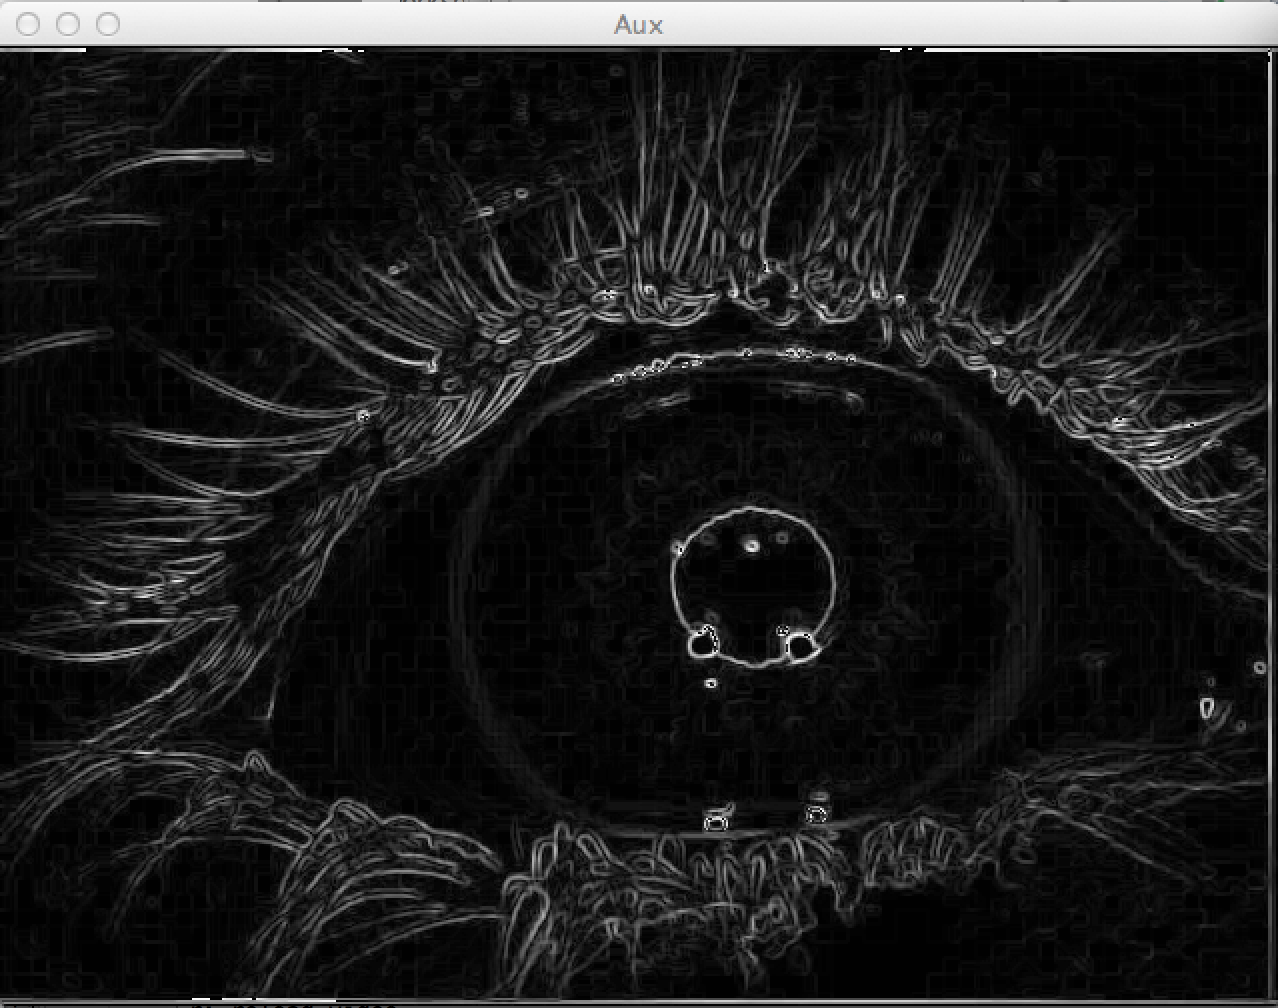
\includegraphics{pics/hough/3.png}
\caption{Our calculated edge magnitude image for a closeup image of an
eye. Brighter spots equals a longer gradient which means a larger
contrast \label{hough3}}
\end{figure}

Thresholding this image will (if we exclude all below the threshold)
give us a set of n pixels, that with high probability is part of a
edge/line in the image. Each of these pixels will produce an infinite
amount of lines in the Hough space. Where a lot of these lines intersect
is a point corresponding to a line in the image space. Each point in
image space, will produce a lot of ``bad'' results, and to filter out
these results the hough algorithm uses a voting system.

\begin{figure}[htbp]
\centering
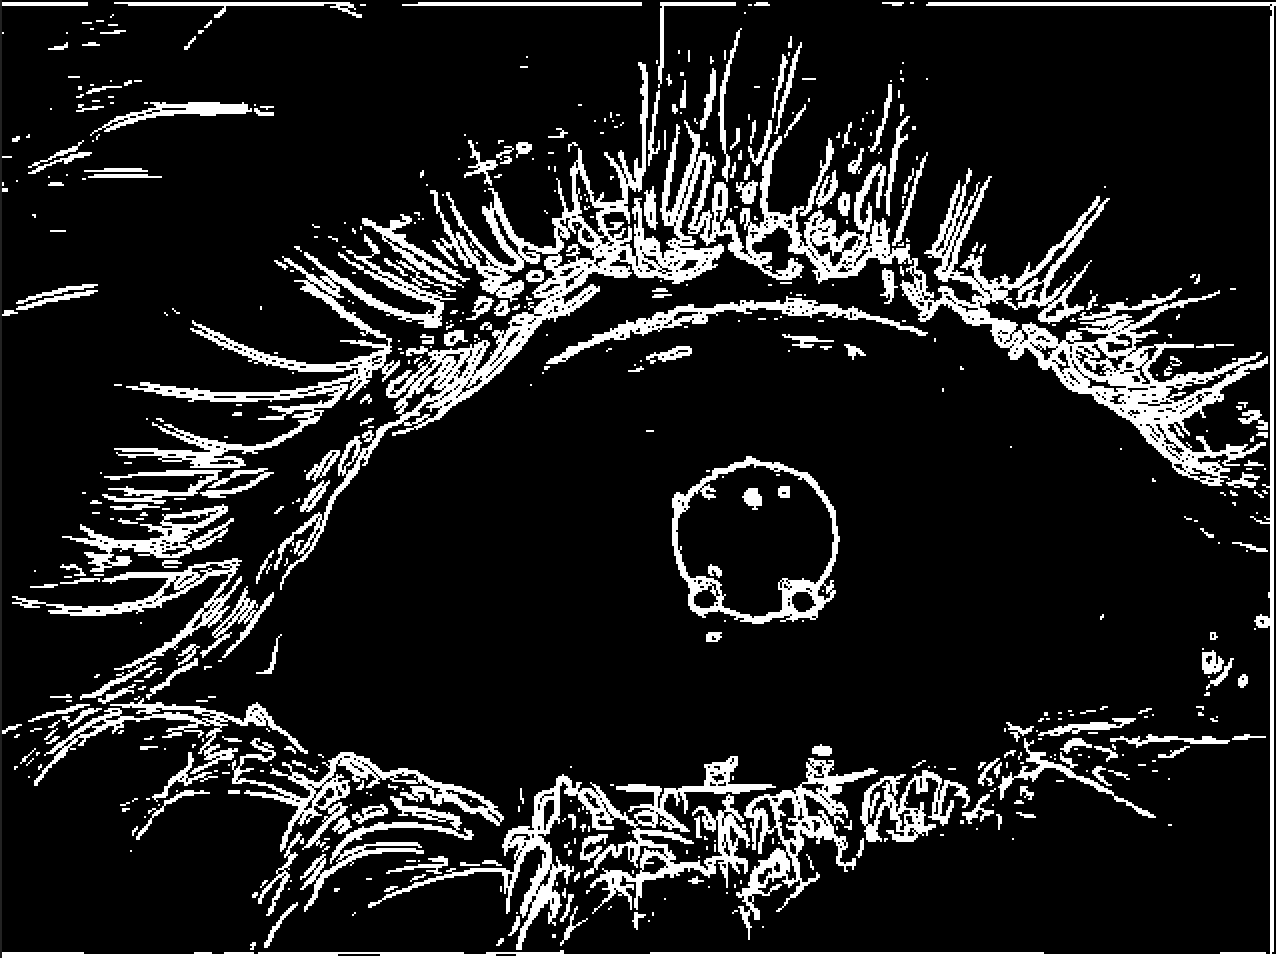
\includegraphics{pics/hough/4.png}
\caption{Thresholded magnitude image \label{hough4}}
\end{figure}

The hough space is quantized into small cells. Each time a line in the
hough space passes through a cell, the value of the cell is increased by
one. We say that the line ``votes'' for that cell. After calculating all
possible votes in the hough space, we'll end up with an accumulated
image, where several points have voted for certain points, thereby
voting for the existence of a line in the image space.

\begin{figure}[htbp]
\centering
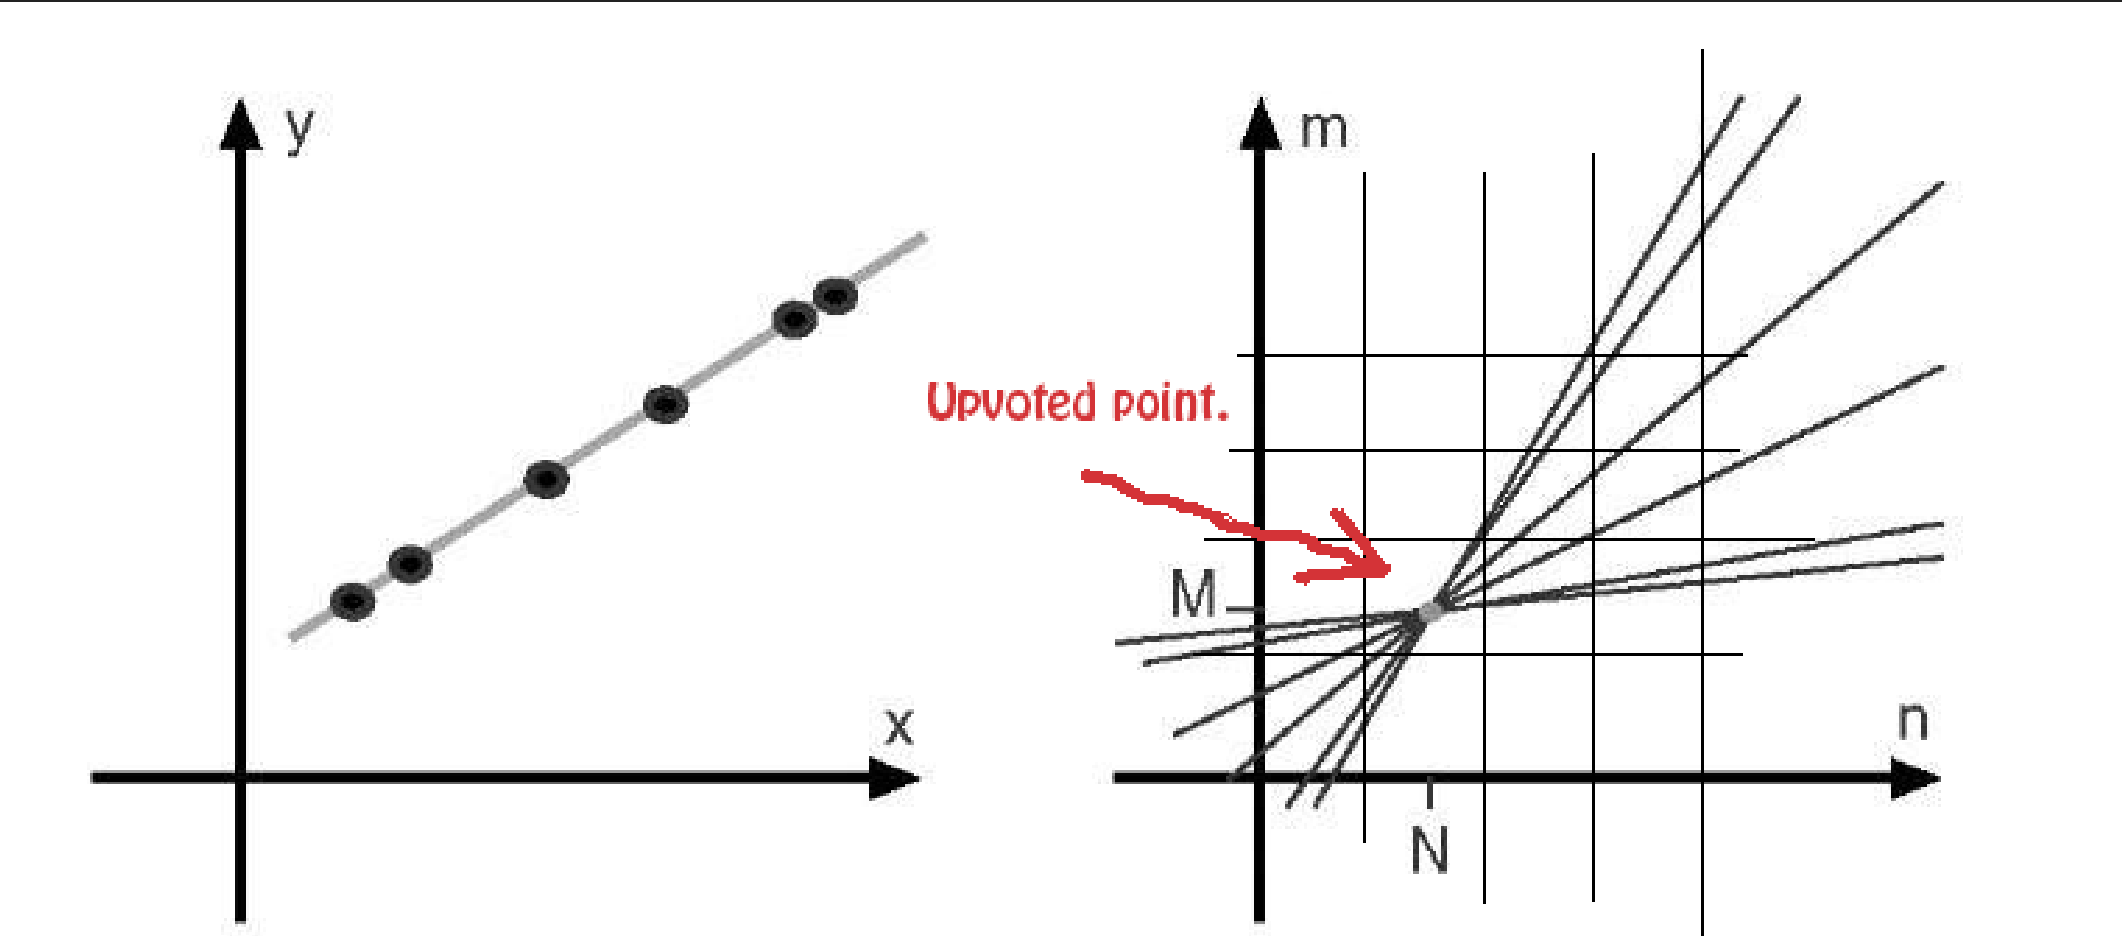
\includegraphics{pics/hough/5.png}
\caption{Upvoted point \label{hough5}}
\end{figure}

\subsection{Polar representation}

Using $b = -mx +y$ as representation in Hough space can be problematic
when dealing with vertical lines, so instead we use the polar
representation where each point in image space (x,y) corresponds to
points on the sinusoid curve
$x_i \cos{ \theta } + y_i \sin{ \theta } = \rho$ in Hough space. The
technique is the same, where each point $( \rho, \theta)$ on the curve
will up-vote points in the accumulated Hough-image $H[ \rho , \theta]$

\begin{figure}[htbp]
\centering
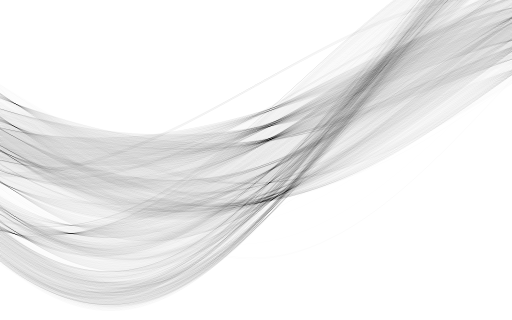
\includegraphics{pics/hough/6.png}
\caption{Hough space sinusoid curve. (Here rather illustrative but alas
not very informative, as it is without coordinates.) \label{hough6}}
\end{figure}

\subsection{Hough Circle Transform:}

In the line detection case, a line was defined by two parameters. In the
circle case, we need three parameters to define a circle.(From OpenCV
documentation.)

$C: (Xcenter, Ycenter, radius)$

The hough-space is therefore also increased by one dimension, to
accommodate the third ``unknown''. Should we wish to find more
sophisticated shapes, the hough space can theoretically be increased by
n dimensions. Although the calculations performed in the voting
algorithm, are expensive and the accumulated cost rise dramatically with
each dimension added.

\textbf{Open CV implementation:}

The openCV method first performs a canny edge detection, and then uses a
bit more complex voting method using the gradient directions to guide
the Hough voting process. (Presumably using the methods we described
earlier , sorting out voting results, where the angle between the
gradient, and the circle normal within a defined threshold. Although the
OpenCv documentation is not quite clear on this point).

\textbf{Our Implementation:}

\begin{verbatim}
def detectPupilHough(gray):
    #The method takes a gray-scale image.
        blur = cv2.GaussianBlur(gray, (81,81), 11)
    #The image is blurred to remove noise, that could potentially create gradiants where there are no edge. Its a fine line though, as the blurring potentially could make it harder to find the edges we're trying to locate.
        slidervals = getSliderVals()
    #This is so we can adjust the min/max radius for accepted circles.
        dp = 6; minDist = 30
    #This determines the resolution of the Hough-space and the minimum distance between found circles.
        highThr = 20
    #As the Cv2 uses canny edge detection, this sets the threshold for accepting “line” pixels.
        accThr = 150;
    #Determins how many votes that a circle should receive to be accepted (and drawn).
        minRadius = slidervals['Hough pupil size']-7;
        maxRadius = slidervals['Hough pupil size']+7;
    #Sets the size of the accepted circles.
        circles = cv2.HoughCircles(blur,cv2.cv.CV_HOUGH_GRADIENT, dp,minDist,                 None, highThr,accThr,minRadius, maxRadius)
    #The actual cv2 method that uses all the parameters just explained.
    #The rest is just drawing the circles (drawing a red circle for the circle with most votes.)
        gColor = cv2.cvtColor(gray, cv2.COLOR_GRAY2BGR)
        if (circles !=None):
                all_circles = circles[0]
                M,N = all_circles.shape
                k=1
                for c in all_circles:
                cv2.circle(gColor, (int(c[0]),int(c[1])),c[2], (int(k*255/M),k*128,0))
                K=k+1
                        c=all_circles[0,:]
                        cv2.circle(gColor, (int(c[0]),int(c[1])),c[2], (0,0,255),5)
cv2.imshow("houghPupil",gColor)
\end{verbatim}
\subsection{Our Results}

Finding the pupil: As with all the methods in this report, the
parameters of the cv2 method had to be adjusted to fit the resolution
and lighting of each video.

\subsubsection{Test 1. Unknown subject closeup.}

figure \ref{hough7} Test settings: Smoothing: gaussian blur, kernel size
(11,11). Circle Threshold: 200.

\begin{figure}[htbp]
\centering
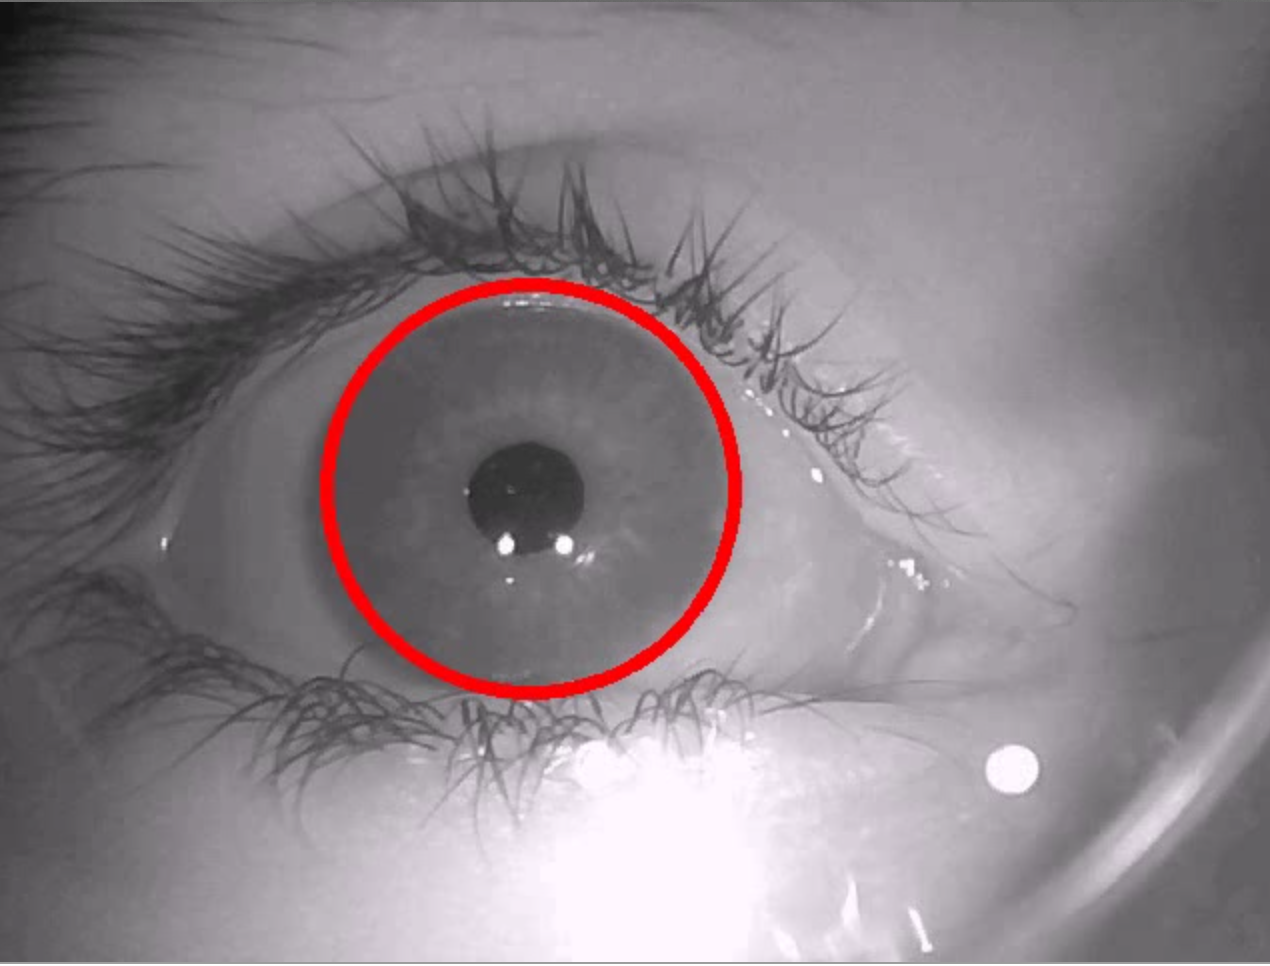
\includegraphics{pics/hough/7.png}
\caption{These circumstances are ideal for detecting the iris, as the
iris itself is highly visible and a lot of high contrast circle poins
help determine the circle placement. The top of the circle may be
detected on the eyelid rather than the iris though, as the contrast
there is larger that on the actual iris. \label{hough7}}
\end{figure}

\begin{figure}[htbp]
\centering
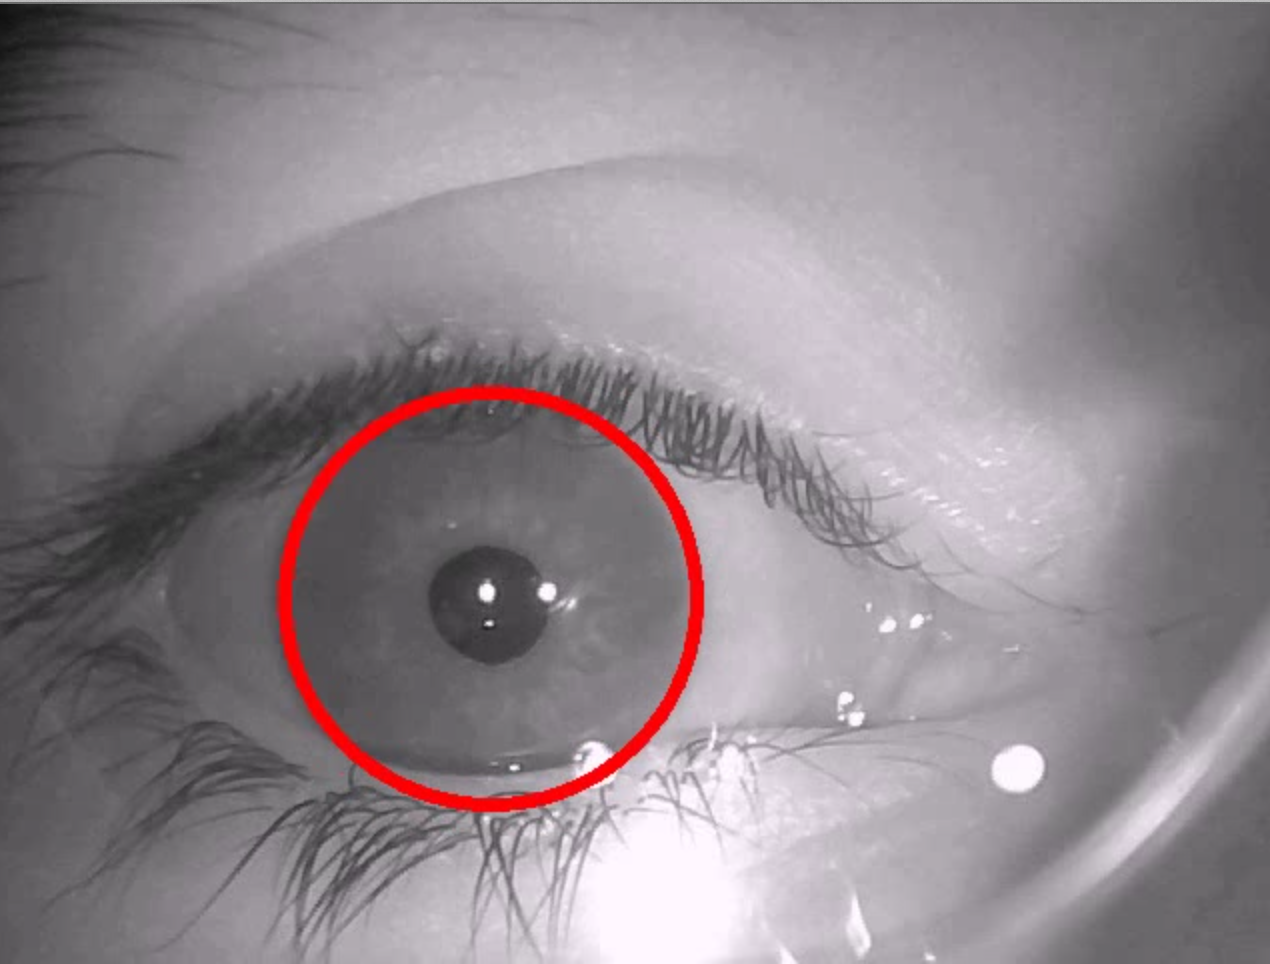
\includegraphics{pics/hough/8.png}
\caption{On this image we se why the hough transformation is really
reliable. The circle is detected even though the eyelids top and bottom
cover some of the iris. The points at the sides makes up for that and
casts enough votes on there being a full circle where the iris is,
therefore overcomming the problem that some of the iris is not visible.
\label{hough8}}
\end{figure}

\begin{figure}[htbp]
\centering
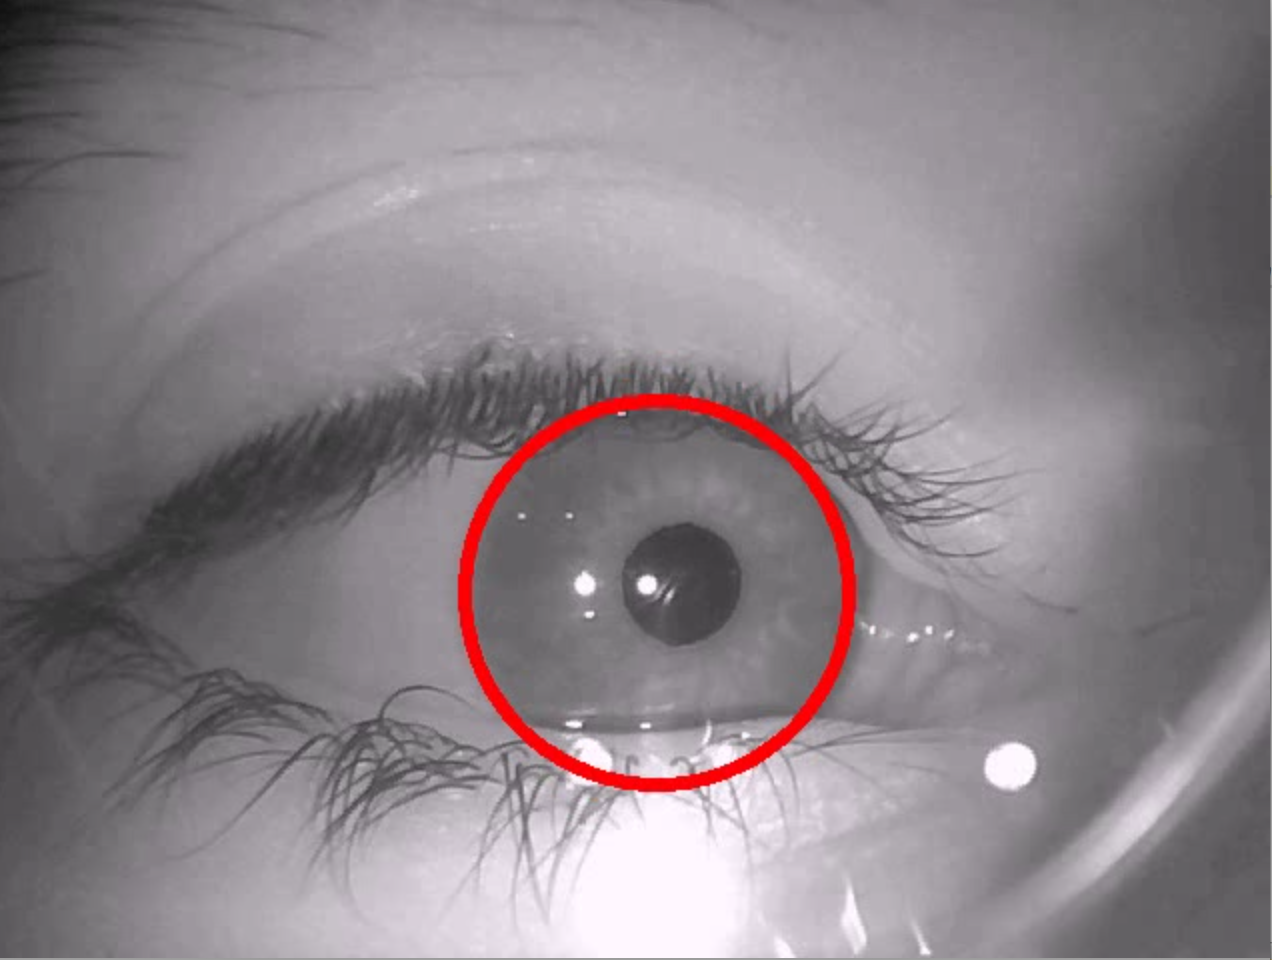
\includegraphics{pics/hough/9.png}
\caption{Even at the sides the method detects a circle, through movement
and other distractions. The circle jumps a lot, as more that one circle
is detected around the iris and they each take turns getting the most
votes, but overall a good result in these ideal circumstances.
\label{hough9}}
\end{figure}

\subsubsection{Test 2. Young Master Roed recorded 12/03/13 Pupil
Detection.}

Test settings: GaussianBlur(gray, (11,11), 11) Threshold : 50 Min/Max
size circle: 10-17

\begin{figure}[htbp]
\centering
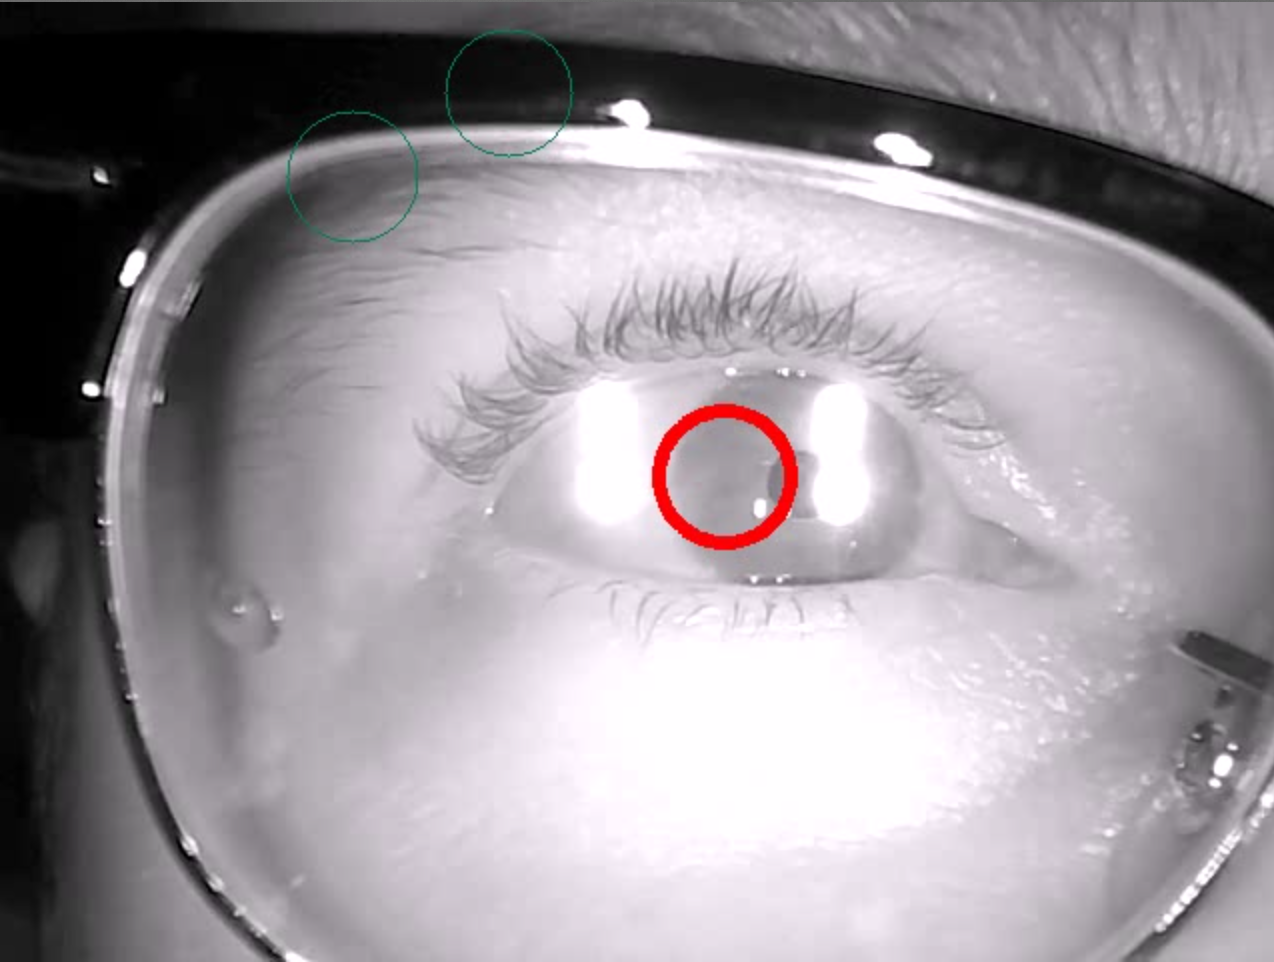
\includegraphics{pics/hough/10.png}
\caption{This image contains many distractions. The infrared lights made
a massive four reflections in the glasses covering the pupil. Instead of
finding the pupil, a part of the iris is detected as a circle edge.
\label{hough10}}
\end{figure}

\begin{figure}[htbp]
\centering
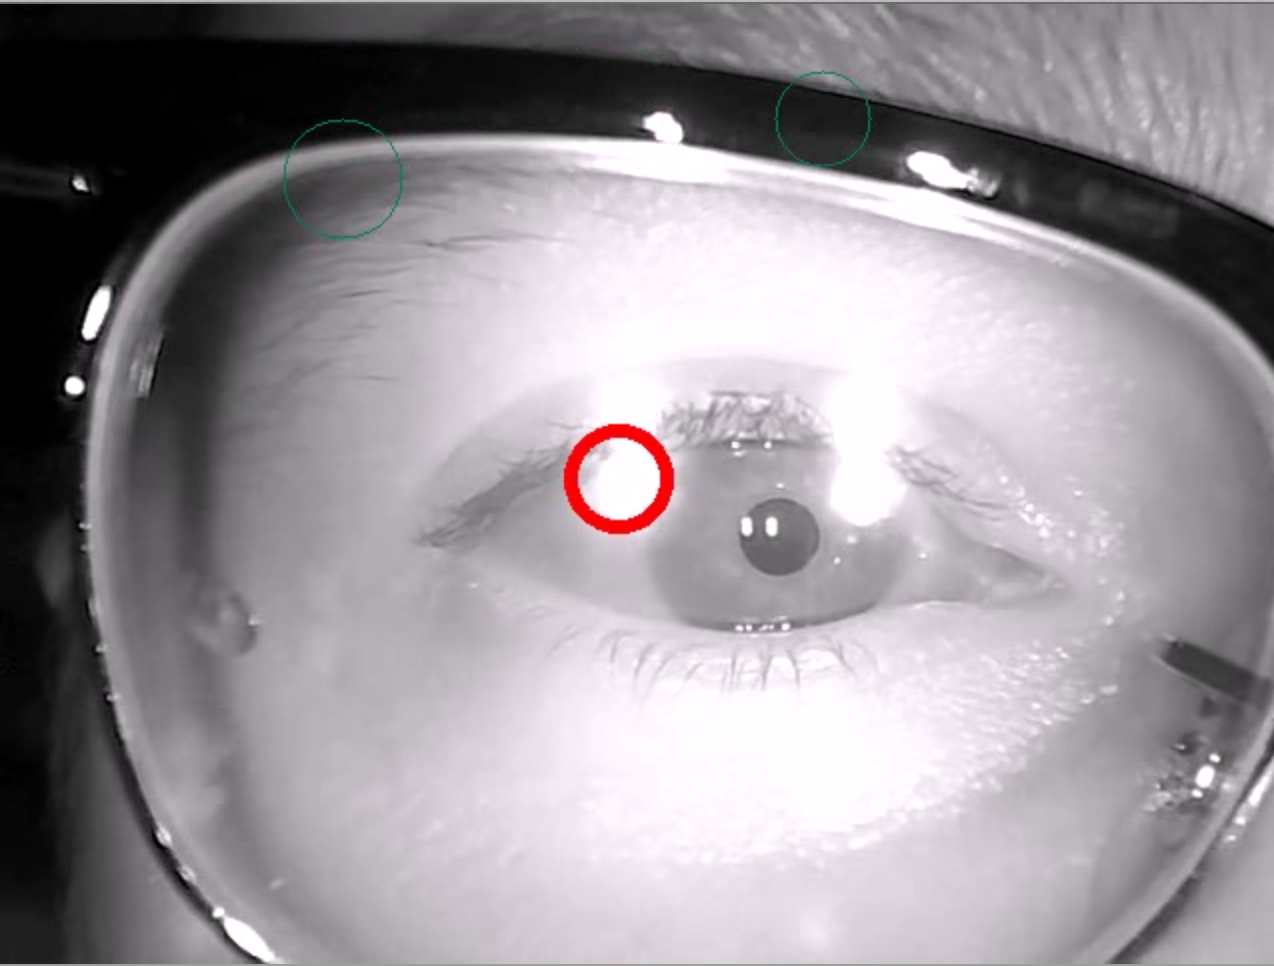
\includegraphics{pics/hough/11.png}
\caption{The distractions keep having an influence on the result, as on
this image, where the best circle match is the circular reflection of
the infrared light. THis could be compensated for by lowering the
threshold ond filtering the bads results afterwards. \label{hough11}}
\end{figure}

\begin{figure}[htbp]
\centering
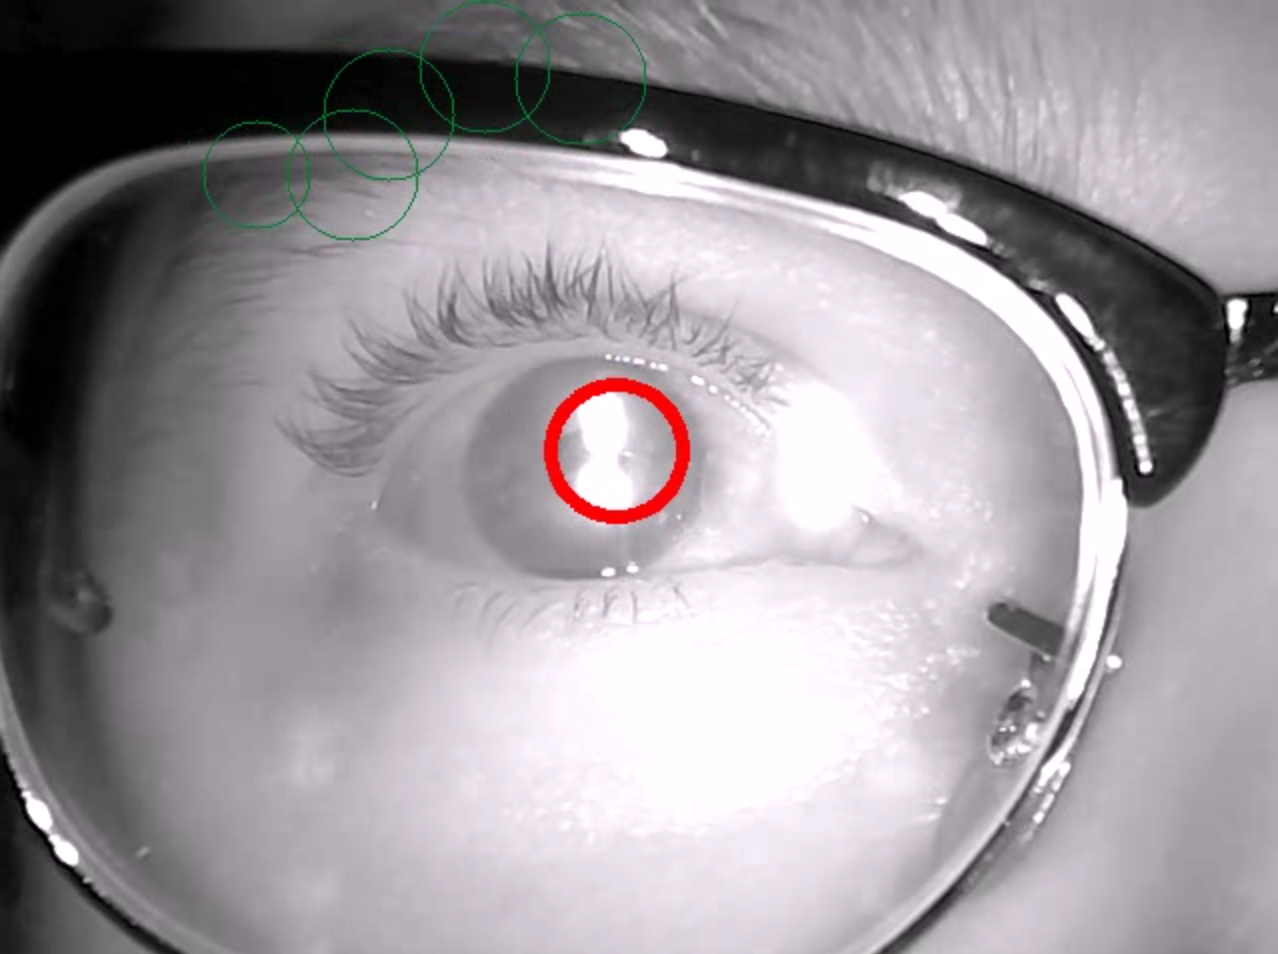
\includegraphics{pics/hough/12.png}
\caption{The distractions just proved to be too large an obstacle, as
the eye movements keeps concealing most of the pupil. Even though the
Hough method is pretty stable, it still requires a bit more controlled
environment. \label{hough12}}
\end{figure}

\subsubsection{Test 3. Young Master Roed recorded 12/03/13 Iris
Detection.}

Test settings: GaussianBlur(gray, (21,21), 11) Threshold : 120 Min/Max
size circle: 30-37

\begin{figure}[htbp]
\centering
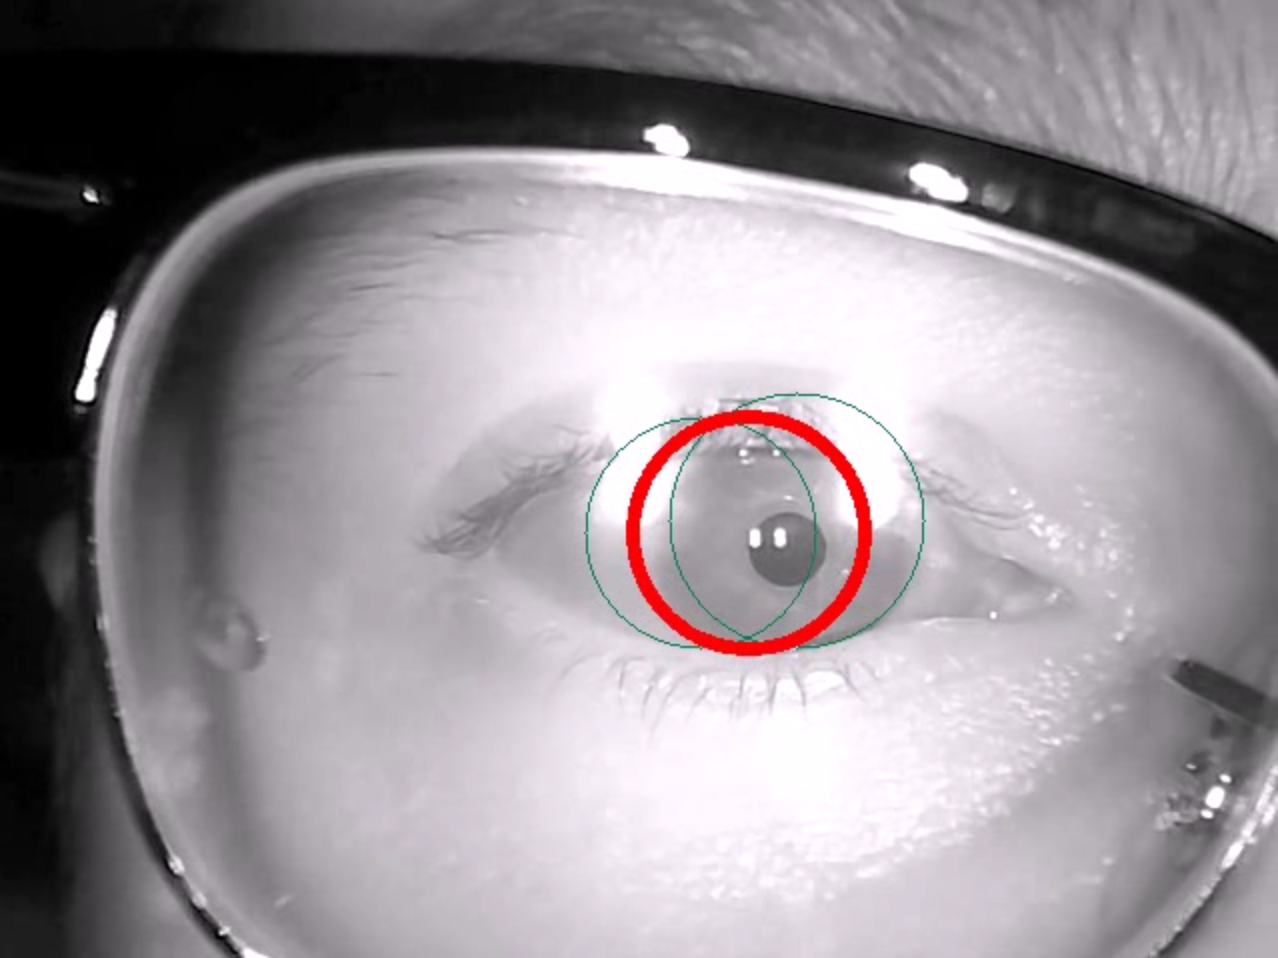
\includegraphics{pics/hough/13.png}
\caption{Finding the pupil proved a bit easier. This i probably because
the iris size is much bigger than the distraction reflection circles.
\label{hough13}}
\end{figure}

\begin{figure}[htbp]
\centering
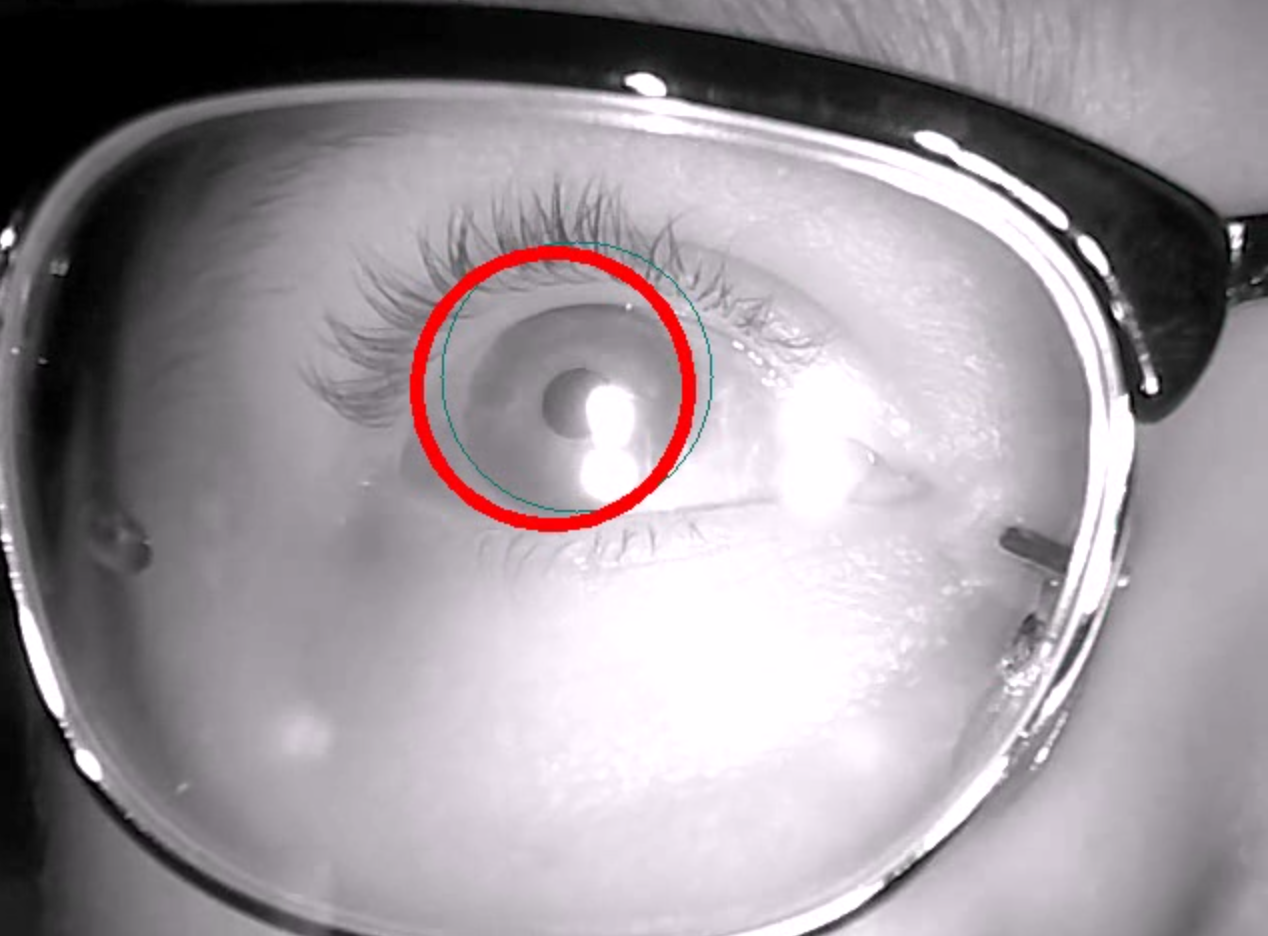
\includegraphics{pics/hough/14.png}
\caption{Looking to the sides will make the circle jump around a lot, as
it can be seen at the video. A lot of the votes still end up pat the
correct spot though. \label{hough14}}
\end{figure}

\begin{figure}[htbp]
\centering
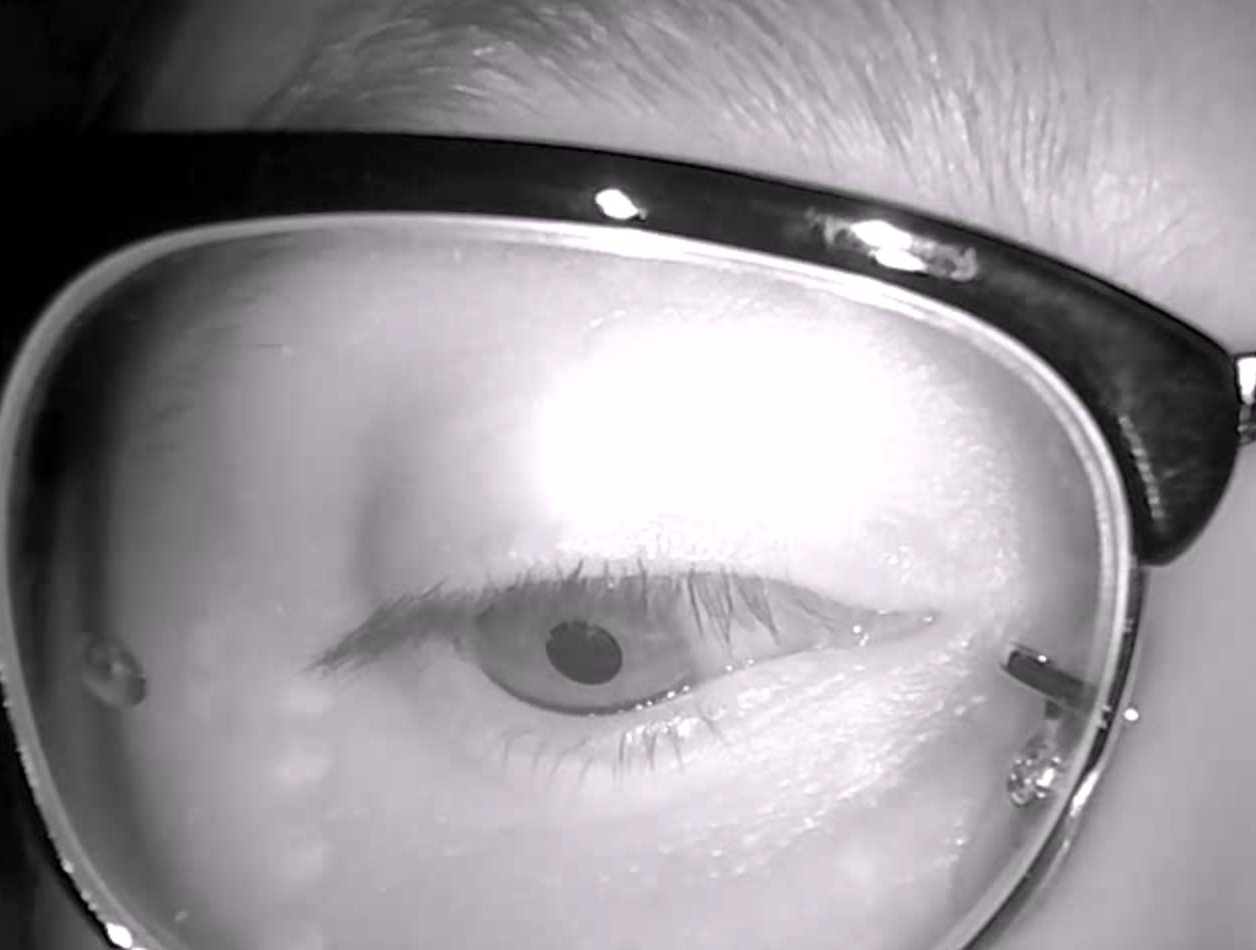
\includegraphics{pics/hough/15.png}
\caption{In this fram, there's just not enought circle edge points
visable to determine the presence of a circle. The right side of the
iris could help, but its just not enought without lowering the threshold
even further. \label{label15}}
\end{figure}

\begin{figure}[htbp]
\centering
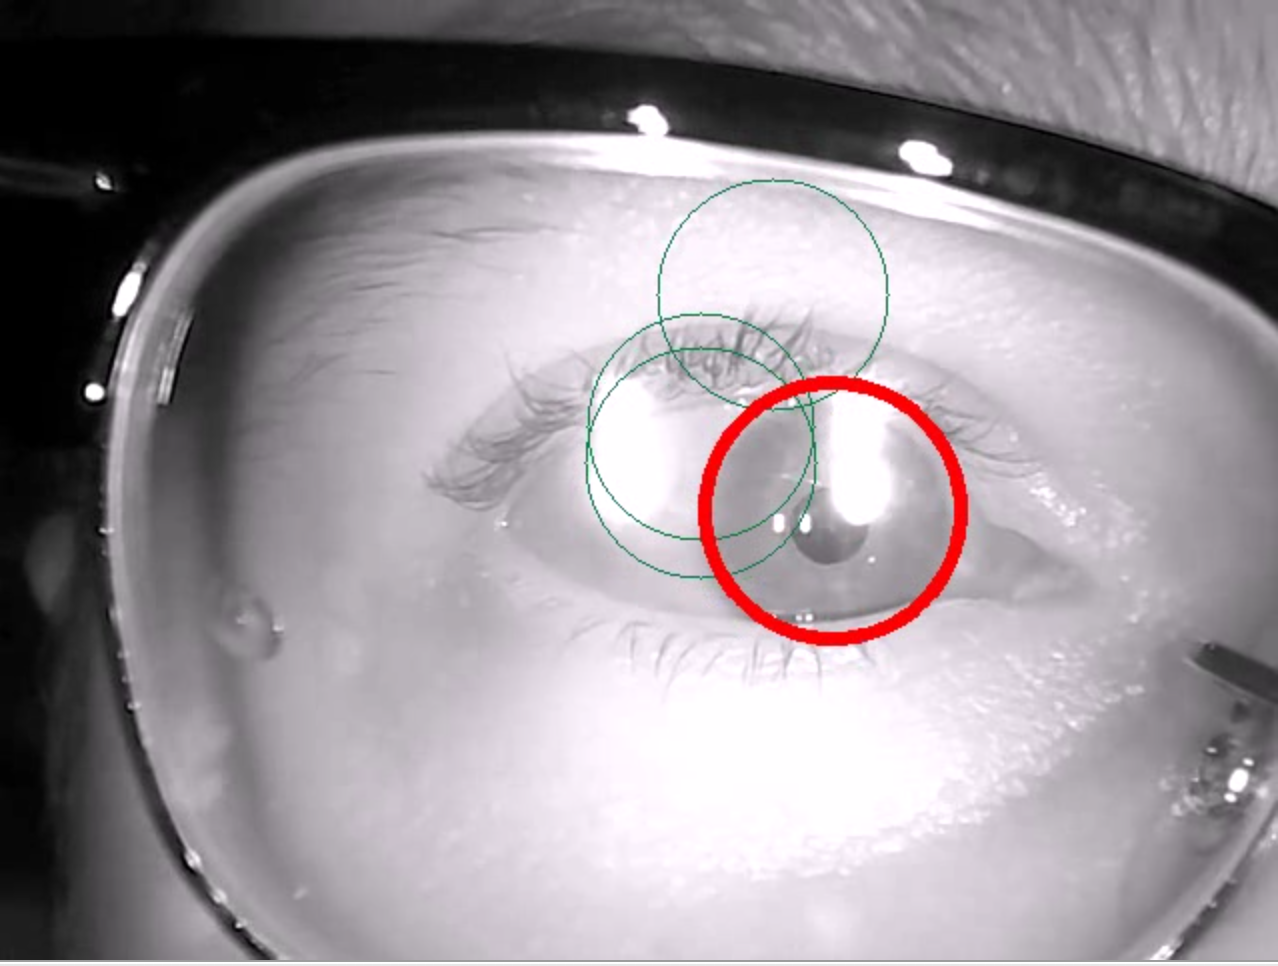
\includegraphics{pics/hough/16.png}
\caption{The threshold has been lowered even further here to 90 and
other circles appear. The most votes are still placed on the correct
circle though. \label{label16}}
\end{figure}

\subsection{Our Impressions of the technique:}

\subsubsection{When does it work?}

In an environment, where you can control the distance, resolution and
lighting of the video/image sequence, the Hough transform is very solid.
The method shines when trying to detect circles that are not complete.
As long as enough points are visible so that the circle-votes pass the
defined threshold, the method will draw the circle. This puts the method
ahead of the competition. When compared to other methods like the
thresholding method, that depends on the circularity of the found blob,
and when looking at solely using the norms for detection, being more
prone to error caused by other high gradients placed on the norm lines,
the Hough transform seems like the way to go for pupil and Iris
detection.

\subsubsection{When does it not work?}

It can be hard to set the correct threshold for the canny edge detection
as well as the minimum votes threshold, to get the correct amount of
circles. If you set it to strict it may look well with optimal
conditions, and then jump to drawing nothing as soon as the conditions
deteriorate. On the other hand, if you are less rigid with the
thresholding and min/max radius, it may look well in one image and then
jump to thousands of found circles in the next image, slowing down the
whole process. When detecting the iris we ran into some problems as
well, as the iris is not so well defined as the pupil. As it can be seen
in the video, the found iris-circle jumps a lot around. This is probably
caused by the lack of iris edge-pixels visible in the image for the
circle. The circle is found only with votes from the sides of the iris,
as the shape of the iris in reality resembles an ellipse, not a circle.

\subsection{Improving the method:}

If we were to improve the method, we would combine it with more of the
other techniques mentioned in this report. We would: Automatically
determining the pupil size with k-mean clustering. Sort out ``wrong''
results with positioning I relation to other features. Use the last
known position to filter out wrong results. (as the video is about 30
frames per second we can estimate the max movement per frame, and filter
out results that lie outside this range.)

\subsection{Conclusion:}

Out of the box, Hough transform works quite well for pupil/iris
detection, its robust even if the image contains noise (salt and pepper,
not large distractions), and when considering that the method allows for
searching for multiple times appearence of a shape in a single pass its
both fast and reliable.
